\documentclass[12pt, dvipdfmx]{beamer}

\renewcommand{\kanjifamilydefault}{\gtdefault}
%%%%%%%%%%%  package  %%%%%%%%%%%
\usepackage{bxdpx-beamer}% dvipdfmxなので必要
\usepackage{pxjahyper}% 日本語で'しおり'したい

\usepackage{amssymb,amsmath,ascmac}

\usepackage{multirow}
\usepackage{bm}

\graphicspath{{../figure/}}

\usepackage{tikz}
\usepackage{xparse}
\usetikzlibrary{shapes,arrows}
%% define fancy arrow. \tikzfancyarrow[<option>]{<text>}. ex: \tikzfancyarrow[fill=red!5]{hoge}
\tikzset{arrowstyle/.style n args={2}{inner ysep=0.1ex, inner xsep=0.5em, minimum height=2em, draw=#2, fill=black!20, font=\sffamily\bfseries, single arrow, single arrow head extend=0.4em, #1,}}
\NewDocumentCommand{\tikzfancyarrow}{O{fill=black!20} O{none}  m}{
\tikz[baseline=-0.5ex]\node [arrowstyle={#1}{#2}] {#3 \mathstrut};}

%目次スライド
% \AtBeginSection[]{
%   \frame{\tableofcontents[currentsection]}
% }
%アペンディックスのページ番号除去
\newcommand{\backupbegin}{
\newcounter{framenumberappendix}
\setcounter{framenumberappendix}{\value{framenumber}}
}
\newcommand{\backupend}{
\addtocounter{framenumberappendix}{-\value{framenumber}}
\addtocounter{framenumber}{\value{framenumberappendix}} 
}

%%%%%%%%%%%  theme  %%%%%%%%%%%
\usetheme{Copenhagen}
% \usetheme{Metropolis}
% \usetheme{CambridgeUS}
% \usetheme{Berlin}

%%%%%%%%%%%  inner theme  %%%%%%%%%%%
% \useinnertheme{default}

% %%%%%%%%%%%  outer theme  %%%%%%%%%%%
\useoutertheme{default}
% \useoutertheme{infolines}

%%%%%%%%%%%  color theme  %%%%%%%%%%%
%\usecolortheme{structure}

%%%%%%%%%%%  font theme  %%%%%%%%%%%
\usefonttheme{professionalfonts}
%\usefonttheme{default}

%%%%%%%%%%%  degree of transparency  %%%%%%%%%%%
%\setbeamercovered{transparent=30}

% \setbeamertemplate{items}[default]

%%%%%%%%%%%  numbering  %%%%%%%%%%%
% \setbeamertemplate{numbered}
\setbeamertemplate{navigation symbols}{}
\setbeamertemplate{footline}[frame number]


\title{絡み合いとプラトー弾性率}
% \subtitle{ ~ はじめに ~}
\author[東亞合成 佐々木]{佐々木 裕\thanks{hiroshi\_sasaki@mail.toagosei.co.jp}}
\institute[東亞合成]{東亞合成株式会社}
\date{\today}

\begin{document}

%%%%%
% 1 P
%%%%%
\maketitle

\section{Z1 code, PPA}
\subsection{Z1 code}
\begin{frame}{Z1 code}
        \centering
            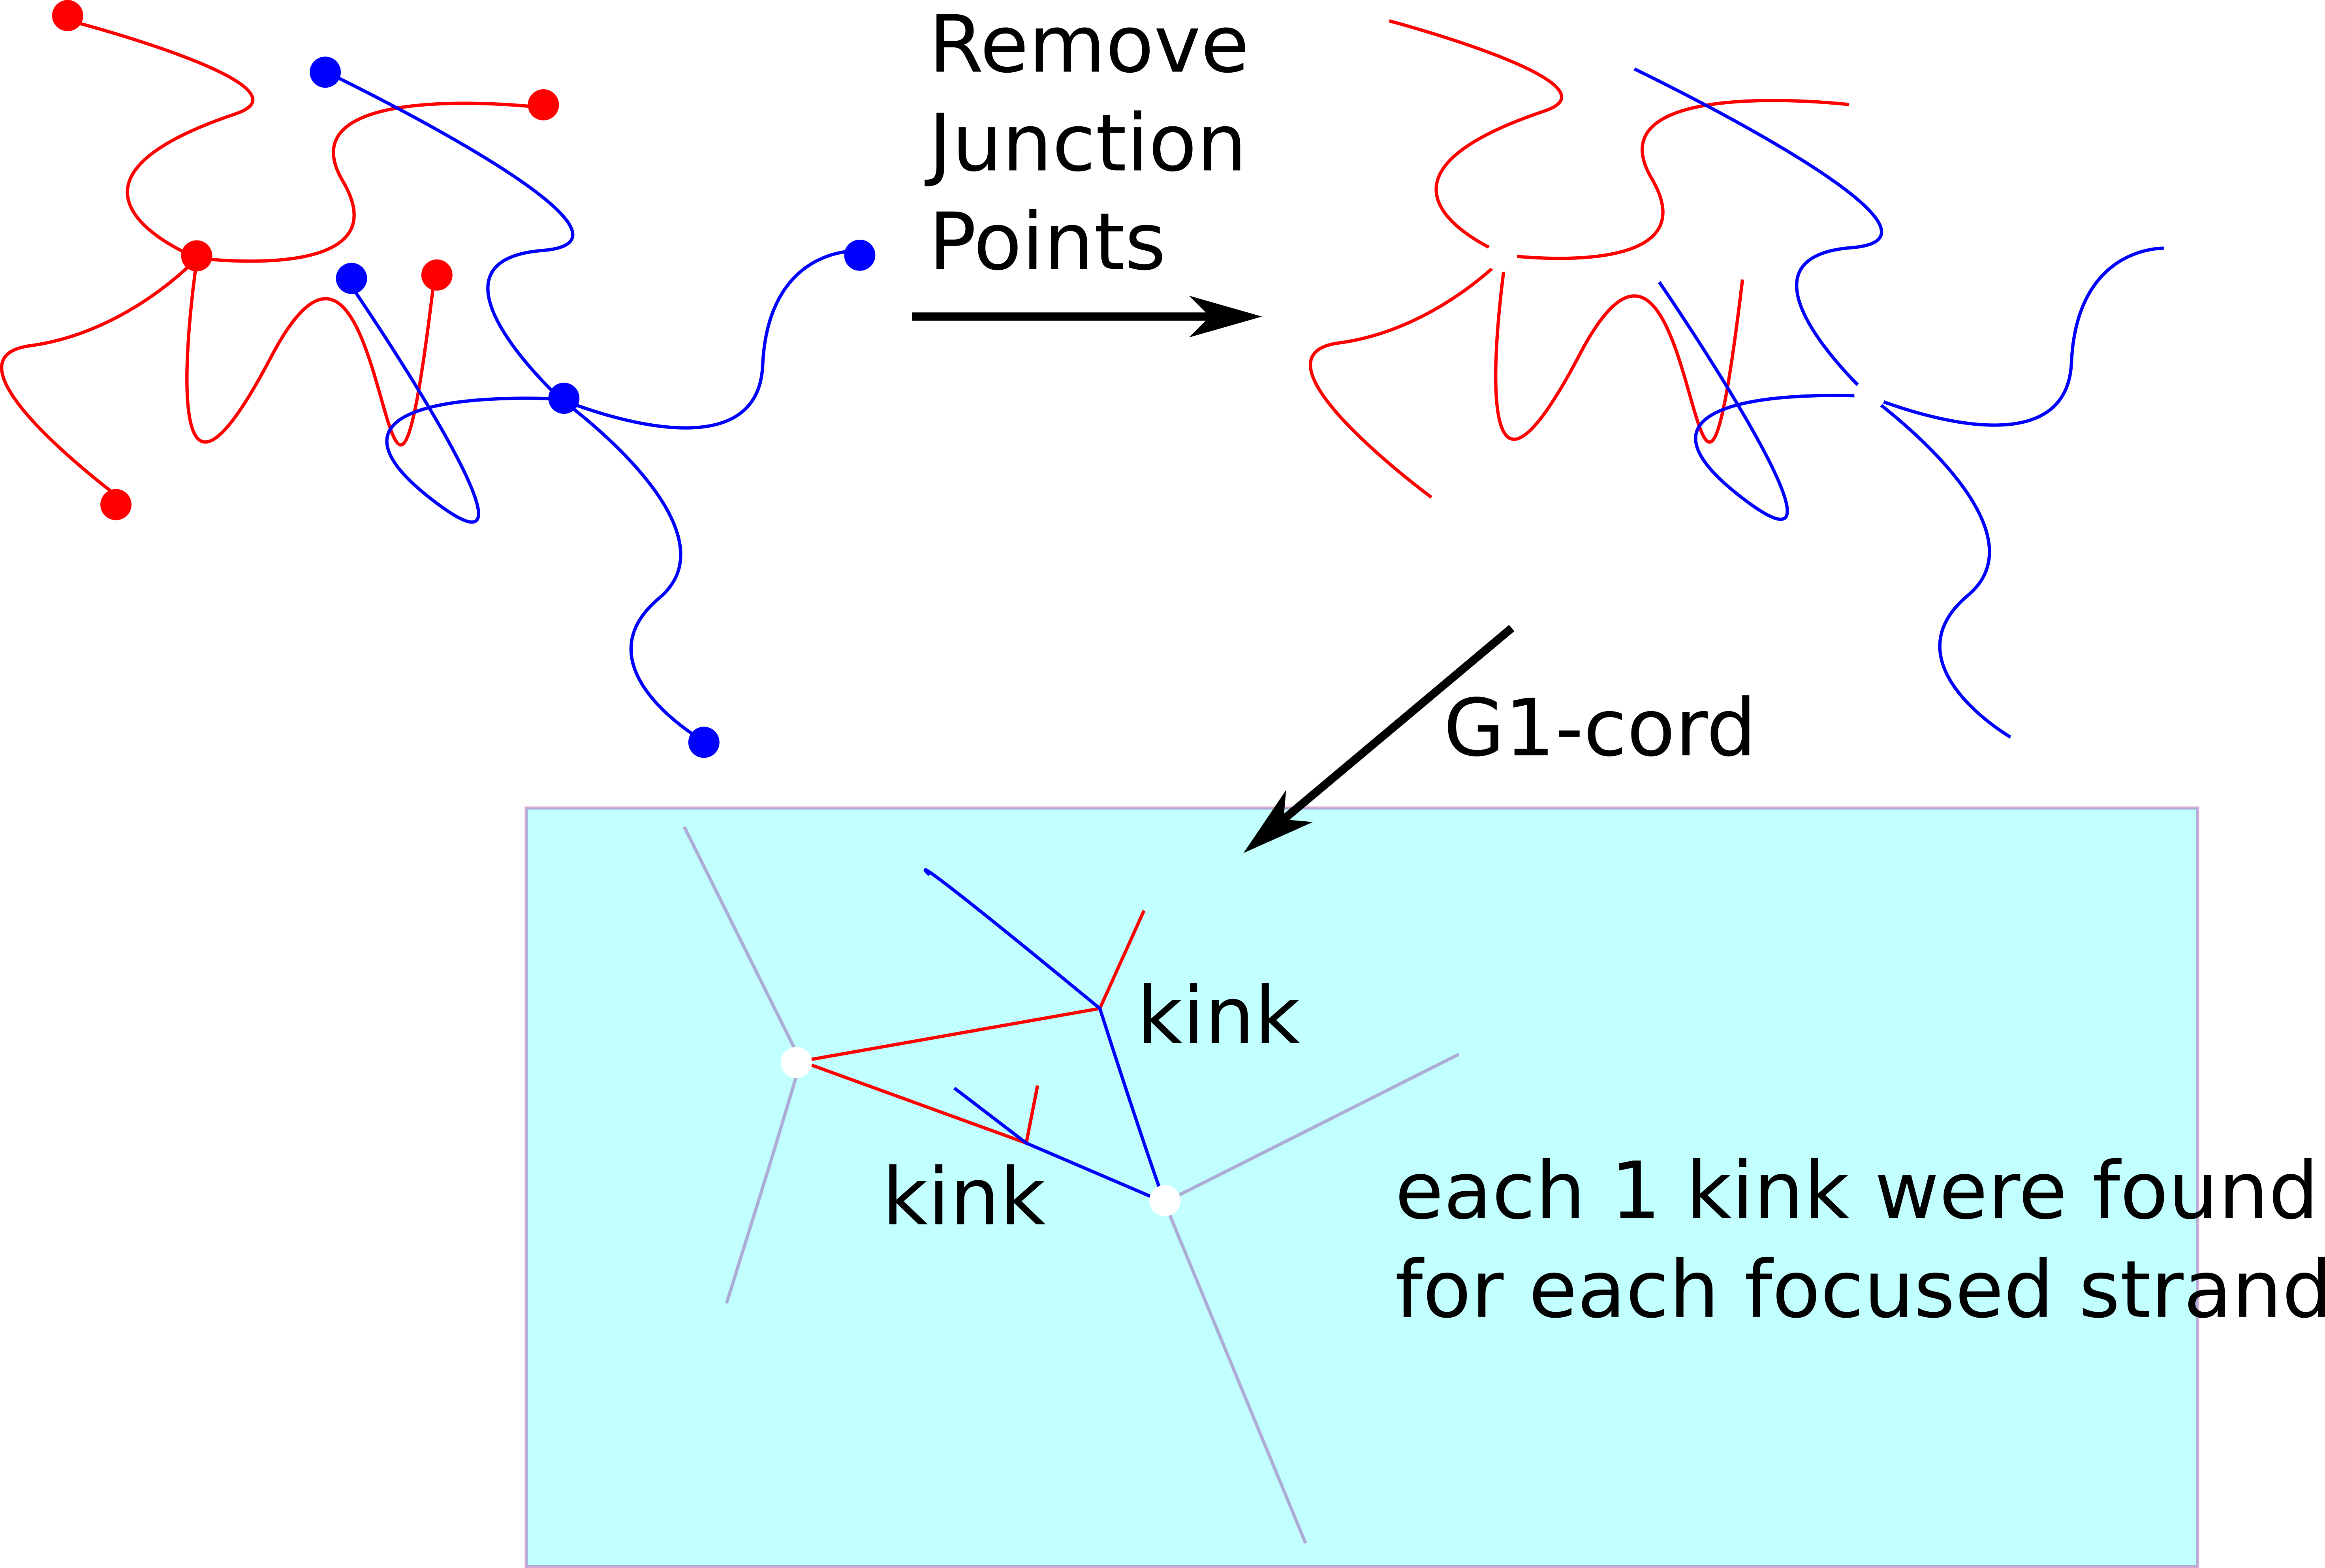
\includegraphics[width=\textwidth]{z1cord.png}
\end{frame} 

\subsection{PPA}
\begin{frame}
    \frametitle{PPA}
    \centering
            \includegraphics[width=.7\textwidth]{z1_PPA.png}
\end{frame}

\subsection{Comparison}
\begin{frame}
    \frametitle{Example for NW}
    \begin{columns}[T, onlytextwidth]
        \column{.28\linewidth}
        \column{.35\linewidth}
        \centering
            Z1 cord
        \column{.35\linewidth}
        \centering
            PPA
    \end{columns}
    \begin{columns}[c, onlytextwidth]
        \column{.28\linewidth}
        NPT\\
        絡み合い小
        \column{.35\linewidth}
        \centering
            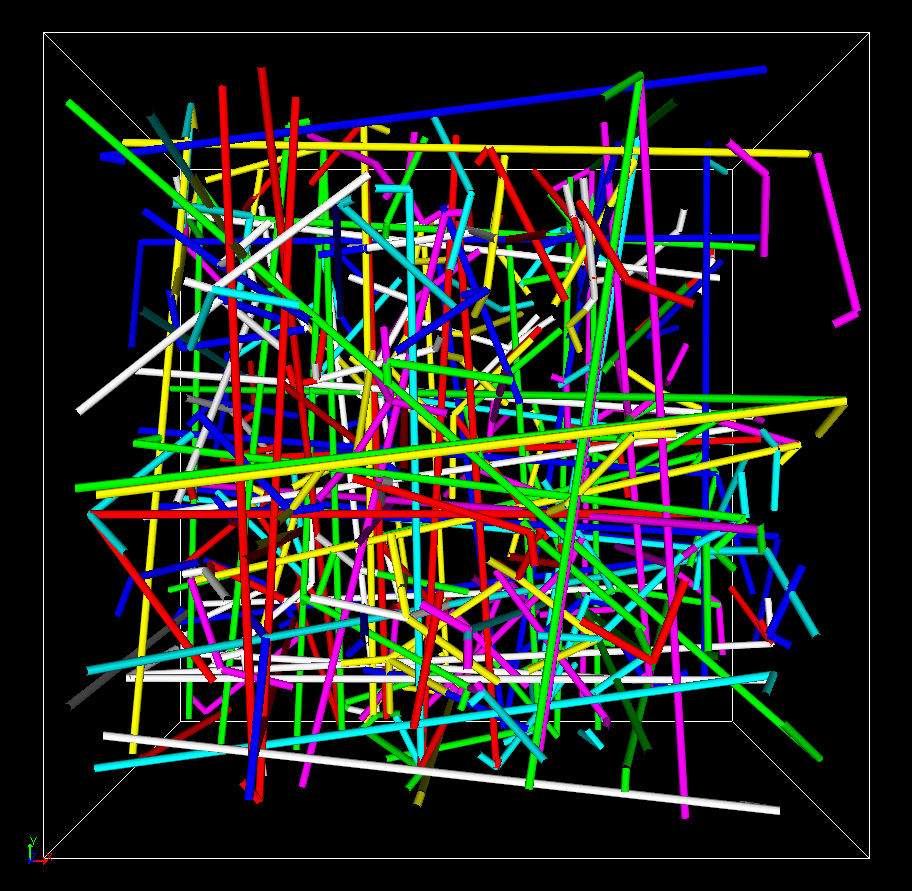
\includegraphics[width=.8\textwidth]{z_cord_NPT_4Chain.png}
        \column{.35\linewidth}
        \centering
            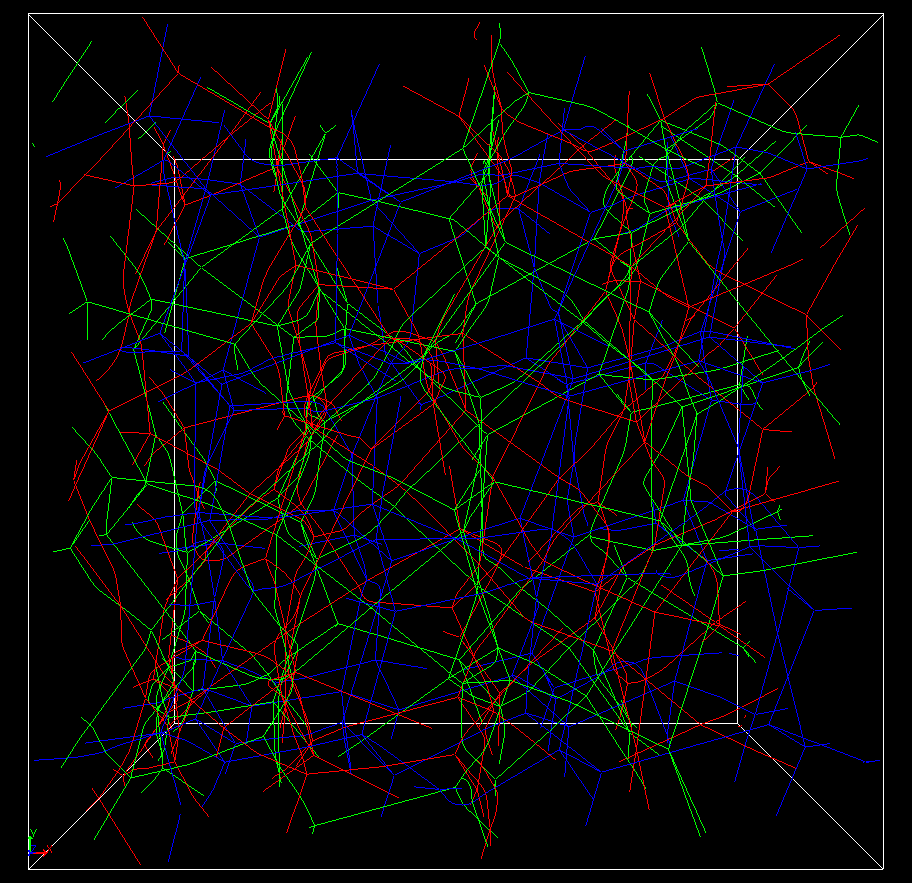
\includegraphics[width=.8\textwidth]{NPT_PPA.png}
    \end{columns}
    \vspace{3mm}
    \begin{columns}[c, onlytextwidth]
        \column{.28\linewidth}
        NVT\\
        自然な絡み合い
        \column{.35\linewidth}
        \centering
            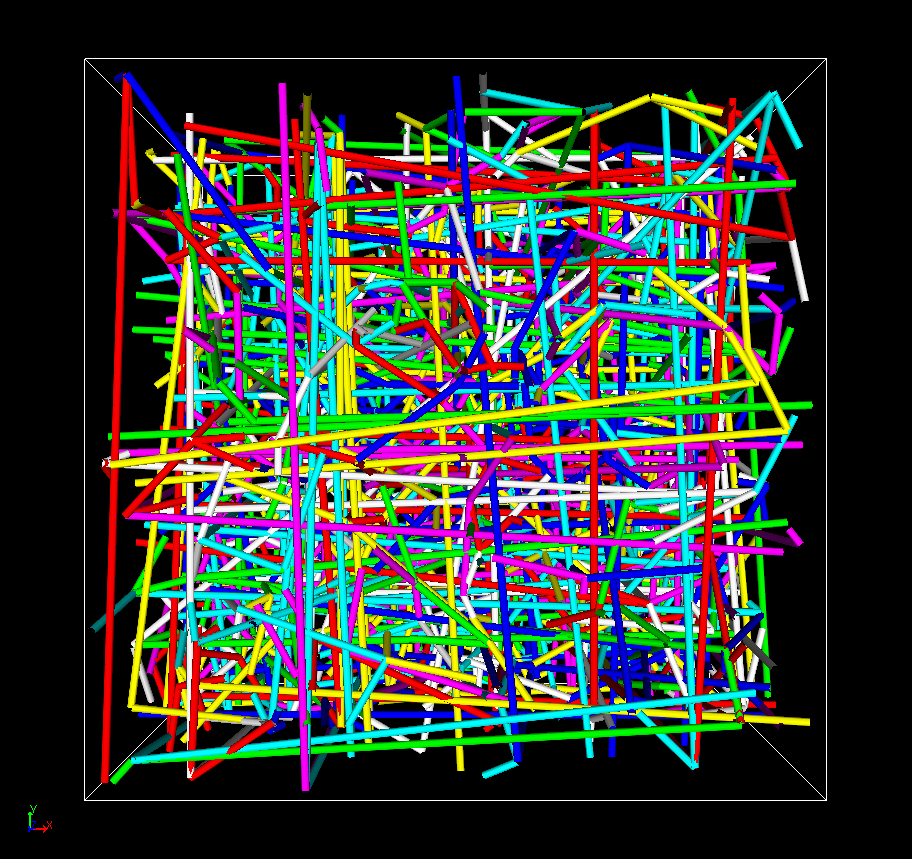
\includegraphics[width=.8\textwidth]{z_cord_4Chain.png}
        \column{.35\linewidth}
        \centering
            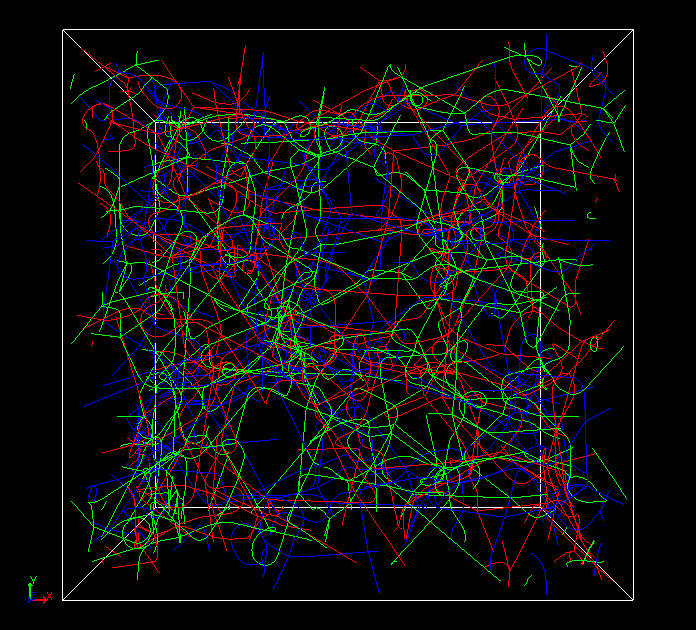
\includegraphics[width=.8\textwidth]{N48_f4_PPA.png}
    \end{columns}
\end{frame}

\end{document}